  % arara: pdflatex

\documentclass[oneside]{article}
\usepackage{pgf-umlsd}
\usepackage{geometry}
\usepackage{float}
\usepackage[simplified]{pgf-umlcd}
\usepackage{hyperref}
\usepackage{minted}

\geometry{letterpaper, margin=1in}

\begin{document}
\title{Free Market Protocol Architecture}
\maketitle

\definecolor{lightyellow}{rgb}{1,1,.92}

The main function of FMP is to transform assets from a `start state' into a `target state' by executing a workflow. Both start state and target state consist of one or more cryptographic assets.  
FMP strives to execute these workflows as efficiently as possible, incurring the least amount of gas fees and slippage as possible, while also requiring a minimal amount of end-user 'approvals' as possible.

\section*{Workflow Domain Model}
The following section provides an overview of the FMP Workflow domain model.
\subsection*{Assets}
FMP Workflow can operate on any of the following kinds assets:

\renewcommand{\umlfillcolor}{yellow!4}
\renewcommand{\umldrawcolor}{black}
\begin{center}
  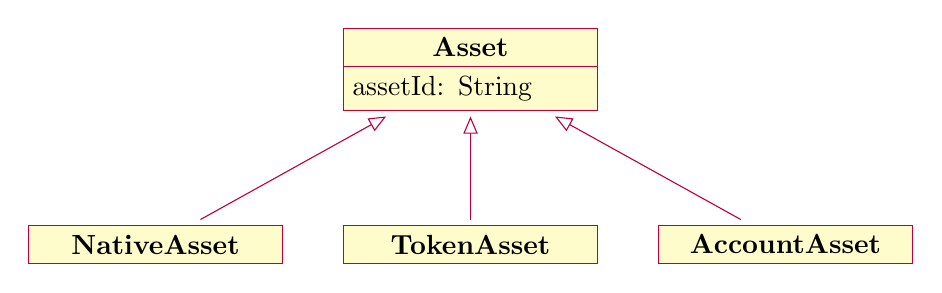
\begin{tikzpicture}[outer sep=2]
    \begin{class}[text width =3 cm]{Asset}{0 ,0}
      \attribute{assetId: String }
    \end{class}
    \begin{class}[text width =3 cm]{NativeAsset}{-4,-2.5}
      \inherit{Asset}
    \end{class}
    \begin{class}[text width =3 cm]{TokenAsset}{0,-2.5}
      \inherit{Asset}
    \end{class}
    \begin{class}[text width =3 cm]{AccountAsset}{4,-2.5}
      \inherit{Asset}
    \end{class}
  \end{tikzpicture}
\end{center}

\begin{itemize}
  \item \textbf{NativeAsset}: The asset that is native to a blockchain, for example Ether (ETH) on Ethereum blockchain, or SOL on Solana.
  \item \textbf{TokenAsset}: A fungible token, for example ``USD Coin" (USDC) which exists as an ERC20 on Ethereum and as an SPL-Token on Solana.
  \item \textbf{AccountAsset}:  An account with some blockchain protocol that holds a balance of some asset.  For example, when a user deposits tokens into a DeX such as DyDx, 
  the tokens are transferred from the user to the exchange, and in return the Dex maintains a balance of those tokens in an account associated with the user. 
\end{itemize}
For simplicity, an account with a negative balance is also modeled as an "asset."  It is not referred to in the model as a liability.

Many assets such (for example USDC) exist on many chains.  In our model, assets are associated with exactly one chain, so for example USDC on Ethereum is considered a different 
asset than USDC on Polygon.

\subsection*{Actions}
Actions are the individual transformation steps within a Workflow.  An action has one or more input assets and one or more output steps, but typically have one input and one output.
\begin{center}
  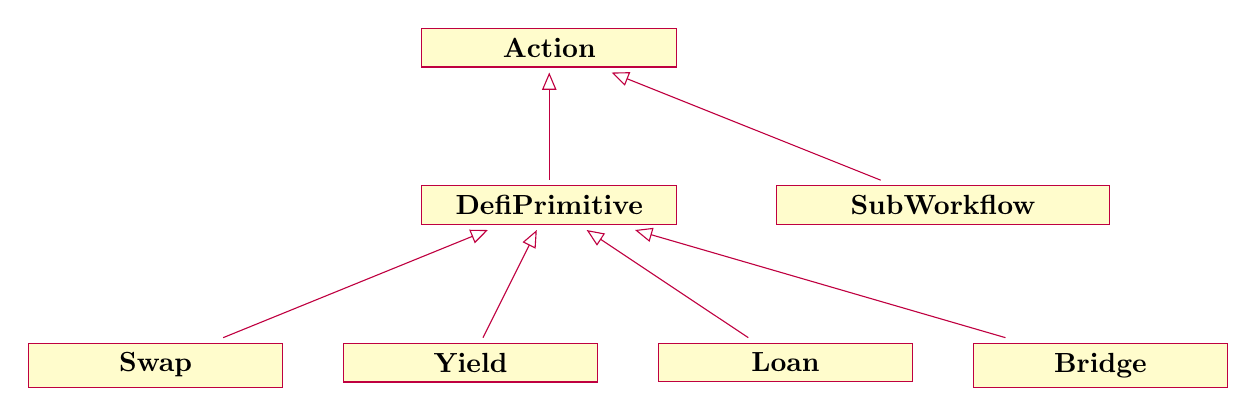
\begin{tikzpicture}[outer sep=2]
    \begin{class}[text width =3 cm]{Action}{0 ,0}
    \end{class}
    \begin{class}[text width =3 cm]{DefiPrimitive}{0,-2}
      \inherit{Action}
    \end{class}
    \begin{class}[text width =4 cm]{SubWorkflow}{5,-2}
      \inherit{Action}
    \end{class}
    \begin{class}[text width =3 cm]{Swap}{-5,-4}
      \inherit{DefiPrimitive}
    \end{class}
    \begin{class}[text width =3 cm]{Yield}{-1,-4}
      \inherit{DefiPrimitive}
    \end{class}
    \begin{class}[text width =3 cm]{Loan}{3,-4}
      \inherit{DefiPrimitive}
    \end{class}
    \begin{class}[text width =3 cm]{Bridge}{7,-4}
      \inherit{DefiPrimitive}
    \end{class}
  \end{tikzpicture}
\end{center}

\begin{itemize}
  \item \textbf{Defi Primitives} are atomic operations within a workflow.  They are implemented by integrating with existing third-party smart contracts.
  \begin{itemize}
    \item \textbf{Swap} A simple swapping from one asset to another, E.g., a workflow action to exchange WBTC for USDC on Uniswap. 
    \item \textbf{Yield} An investment that generates returns over time. E.g., adding liquidity to an Automatic Market Maker pool such as Curve's 3Pool.  
    \item \textbf{Loan}:  Providing collateral using one asset and borrowing a different asset.  E.g., using USDC as collateral on Aave and borrowing BNB.
    \item \textbf{Bridge}:  Transferring assets from one blockchain to another.  For example, using Wormhole to transfer USDC from Ethereum to Avalanche.
  \end{itemize}
  \item \textbf{Sub Workflow} Since workflows have inputs and outputs (described in the next section), workflows can be nested inside of each other.
\end{itemize}

\subsubsection*{Action Notes}
\begin{itemize}
  \item The possible set input asset(s) for a given action are restricted to assets that that particular Action supports.  For example, a Curve 3Pool Swap action 
  can only accept USDT, USDC, or DAI as an input asset. 
  \item Some Actions require additional configuration parameters, which are provided as an Action is included in a workflow.
  \item The output asset(s) is not configured explicitly, but is inferred by the Action's input asset(s) as well as any additional configuration parameters required by the Action.
\end{itemize}

\subsection*{Branches}

A common pattern in DeFi workflows is to repeat a sequence of steps until some desired outcome is achieved.  
To support this, Branches allow flow of execution to be determined by evaluating a boolean expression against data contained in the workflow at runtime.  

\subsection*{Workflows}
Workflows represent configuration of reusable asset transformation logic using the elements described above.  The definition of a workflow consists of:
\begin{itemize}
  \item One \textit{Input Assets} that represent the starting point of the workflow.  
  The amount of that asset is set at execution time, it is not part of the workflow definition. 
  \item A directed graph of nodes, where the nodes consist of \textit{Actions} and \textit{Branches}.  
\end{itemize}

\section*{System Components}
Free Market Protocol consists of the following components:
\\
\\
\noindent \textbf{FMP-SDK}:  A high level programmatic interface enabling developers to easily integrate with the FMP system. FMP-SDK is written in Typescript and runs in the browser and NodeJS, allowing integration of FMP into web based UIs and stand-alone backend systems.
\\
\\
\noindent \textbf{Workflow Solver}:  Given a start-state and a target-state, Workflow Solver will generate a sequence of low level workflow steps to transform the user's starting portfolio to the target portfolio.  Workflow Solver is aware of approximate gas costs and slippage, and produces a workflow that minimizes these costs. 
\\
\\
\noindent \textbf{Workflow Engine}:  Using the workflow steps generated by Workflow Solver, Workflows Engine executes the steps on-chain.  
There is a separate implementation of Workflow Engine deployed on each supported blockchain.  
Workflow Engine carries out the low level workflow steps by invoking with 3rd party contracts. 
All steps in a workflow are executed within a single transaction.

\subsection*{Component Interactions}

The following illustrates a simple scenario and describes the interactions between the various components.  
In this scenario, a user starts with USDC in their Ethereum wallet, and they would like compose a new portfolio earning yield from Curve.fi on the Ethereum blockchain, and Solend on Solana.
\\
\\
First, FMP-SDK passes \emph{startState} and \emph{targetState} to Workflow Solver, representing the user's starting target crypto portfolios respectively.  Workflow Solver then returns a complete set of low level workflow steps.  Note that the workflow contains the required steps accross all blockchains involved in the portfolio transformation:

% \begin{figure}[ht]
%   \begin{sequencediagram}
%     \newthread{A}{FMP SDK}{}
%     \newinst[1]{B}{\shortstack{FMP\\Solver}}{}
%     \newinst[1]{C}{\shortstack{FMP\\Workflow\\Engine\\(ethereum)}}{}
%     \newinst[1]{D}{\shortstack{DEX\\(curve.fi)}}{}
%     \newinst[1]{E}{\shortstack{Bridge\\(wormhole)}}{}
%     \newinst[1]{F}{\shortstack{FMP\\Workflow\\Engine\\(solana)}}{}
%     \newinst[1]{G}{\shortstack{DEX\\(solend)}}{}
%     % \begin{call}{A}{getWorkflow(...)}{B}{}
%     \begin{call}{A}{ getWorkflow(...) }{B}{ workflow }
%     \end{call}
%     \begin{call}{A}{ execute(workflow-eth)}{C}{wormhole-VAA}
%       \begin{call}{C}{ addLiquidity(...)}{D}{lpToken}
%       \end{call}  
%       \begin{call}{C}{ transfer(lpToken,solend)}{E}{wormhole-VAA}
%       \end{call}  
%     \end{call}
%     \begin{messcall}{A}{ execute(workflow-sol, wormhole-VAA)}{F}
%       \begin{call}{F}{ redeem(VAA)}{E}{wh-lpToken}

%       \end{call}  
%       \begin{messcall}{F}{ addLiq(wh-lpToken)}{G}

%       \end{messcall}  
      
%     \end{messcall}
%   \end{sequencediagram}
% \end{figure}

\begin{figure}[H]
  \begin{sequencediagram}
    \tikzstyle{inststyle}+=[top color=lightyellow, bottom color=lightyellow]
    \newthread{A}{FMP SDK}{}
    \newinst[5]{C}{\shortstack{FMP Solver}}{}
    \begin{call}{A}{ \texttt{getWorkflow(}\emph{startState, endState}\texttt{)}}{C}{ \emph{workflow} }
    \end{call}
  \end{sequencediagram}
\end{figure}

\noindent Next, FMP-SDK passes \emph{workflow} to the Workflow Engine to execute the Ethereum part of the workflow:
\begin{figure}[H]
  \begin{sequencediagram}
    \tikzstyle{inststyle}+=[top color=lightyellow, bottom color=lightyellow]
    \newthread{A}{FMP SDK}{}
    \newinst[2.5]{C}{\shortstack{Workflow\\Engine\\(ethereum)}}{}
    \tikzstyle{inststyle}+=[top color=white, bottom color=white ]
    \newinst[2.5]{D}{\shortstack{DEX\\(curve.fi)}}{}
    \newinst[2.5]{E}{\shortstack{Bridge\\(wormhole)}}{}
    \postlevel
    \begin{call}{A}{ \texttt{execute(}\emph{workflow}\texttt{)}}{C}{\emph{VAA}}
      \begin{call}{C}{ \texttt{addLiquidity(}\emph{USDC}\texttt{)}}{D}{\emph{yToken} (curve)}
      \end{call}
      \postlevel
      \begin{call}{C}{ \texttt{wrap(}\emph{yToken}\texttt{)}}{C}{\emph{fmp-yToken}}
      \end{call}        
      \postlevel
      \begin{call}{C}{ \texttt{transfer(}\emph{fmp-yToken, solend}\texttt{)}}{E}{\emph{VAA} (wormhole)}
      \end{call}  
    \end{call}
  \end{sequencediagram}
\end{figure}

In the scenario above, Workflow Engine first invokes Curve's addLiquidity method, providing USDC.  Curve returns some quantity of \emph{yToken}.  
In the next step, Workflow Engine wraps the \emph{yToken}, creating a \emph{fmp-yToken}.  In the last step, the \emph{fmp-yToken} is sent to Wormhole to be transferred to Solana.  
The \emph{VAA} returned by wormhole a token needed to redeem the fmp-yToken on Solana.  Note that this entire portion of the workflow happens on-chain and within a single transaction.  
As such, only one approval is needed from the user to execute all the steps in this workflow.  Also, the workflow steps execute as an atomic unit;  either all steps succeed or the entire transaction is discarded.
\\
\\
\noindent FMP-SDK continues the workflow by invoking the Workflow Engine on Solana:
\begin{figure}[H]
  \begin{sequencediagram}
    \tikzstyle{inststyle}+=[top color=lightyellow, bottom color=lightyellow]
    \newthread{A}{\shortstack{ FMP SDK }}
    \newinst[1.7]{F}{\shortstack{Workflow\\Engine\\(solana)}}{}
    \tikzstyle{inststyle}+=[top color=white, bottom color=white ]
    \newinst[1.7]{E}{\shortstack{Bridge\\(wormhole)}}{}
    % \newinst[2]{H}{\shortstack{DEX\\(saber)}}{}
    \newinst[1.7]{G}{\shortstack{Lender\\(solend)}}{}
    \newinst[1.7]{H}{\shortstack{User's Wallet}}{}
    \postlevel
    \begin{messcall}{A}{\texttt{execute(}\emph{workflow}\texttt{)}}{F}
      \begin{call}{F}{\texttt{redeem(}\emph{VAA}\texttt{)}}{E}{\emph{wh-fmp-yToken}}
      \end{call}  
      % \postlevel
      % \begin{call}{F}{\texttt{swap(}\emph{wh-lpToken}\texttt{)}}{H}{\emph{USDC}}
      % \end{call}  
      \postlevel
      \begin{call}{F}{\texttt{addLiquidity(}\emph{wh-fmp-yToken}\texttt{)}}{G}{\emph{cToken} (solend)}
      \end{call}  
      \postlevel
      \begin{messcall}{F}{\texttt{transfer(}\emph{cToken}\texttt{)}}{H}
      \end{messcall}  
    \end{messcall}
  \end{sequencediagram}
\end{figure}
In the Solana portion of the workflow, Workflow Engine redeems the \emph{fmp-yToken} which is now also wrapped by Wormhole (\emph{wh-fmp-yToken}).  
In the next step this is deposited into Solend in exchange for Solend's \emph{cToken}.  In the final step the \emph{cToken} is transferred to the user's Solana wallet.

\section*{Deployment Architecture}

The following diagram provides an example of how FMP smart contracts are deployed on-chain.  Given that our target for or initial MVP release is EVM compatible blockchains, this diagram is specific to EVM.

\begin{center}
  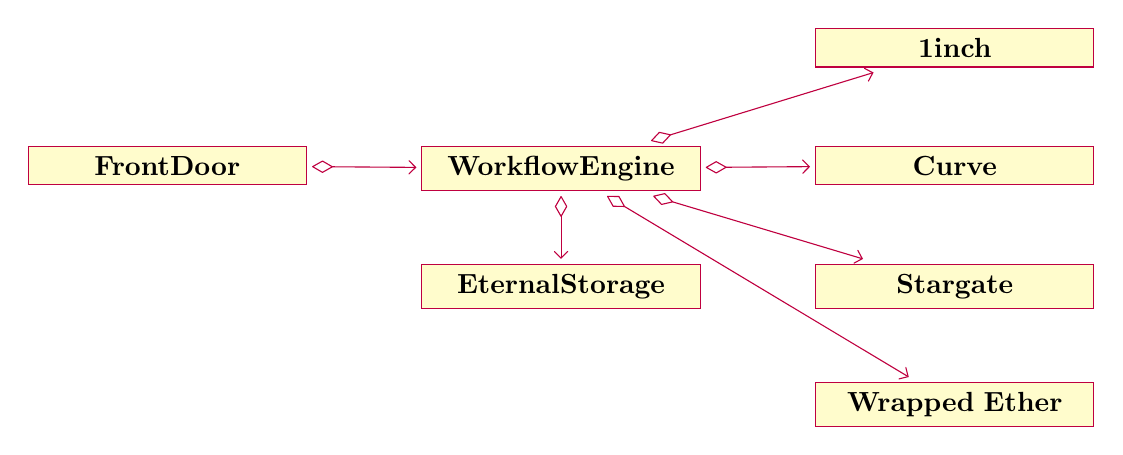
\begin{tikzpicture}[outer sep=2]
    \begin{class}[text width =3.3 cm]{FrontDoor}{0 ,0}
    \end{class}
    \begin{class}[text width =3.3 cm]{WorkflowEngine}{5,0}
    \end{class}
    \begin{class}[text width =3.3 cm]{EternalStorage}{5,-1.5}
    \end{class}
    \begin{class}[text width =3.3 cm]{1inch}{10,1.5}
    \end{class}
    \begin{class}[text width =3.3 cm]{Curve}{10,0}
    \end{class}
    \begin{class}[text width =3.3 cm]{Stargate}{10,-1.5}
    \end{class}
    \begin{class}[text width =3.3 cm]{Wrapped Ether}{10,-3}
    \end{class}
    \aggregation{FrontDoor}{}{}{WorkflowEngine}
    \aggregation{WorkflowEngine}{}{}{1inch}
    \aggregation{WorkflowEngine}{}{}{Curve}
    \aggregation{WorkflowEngine}{}{}{Stargate}
    \aggregation{WorkflowEngine}{}{}{Wrapped Ether}
    \aggregation{WorkflowEngine}{}{}{EternalStorage}
  \end{tikzpicture}
\end{center}

\noindent Each box in the diagram represents a separatly deployed contract.
\\
\\
\noindent \textbf{FrontDoor}:  This contract is the entry point for external callers.  It provides a stable address and is not upgradable.  
It contains the address of the current version of the  WorkflowEngine and simply delegatecalls all transactions to it.
\\
\\
\noindent \textbf{WorkflowEngine}:  Contains the logic for parsing workflow definitions and carrying out the on-chain invocations.
\\
\\
\noindent \textbf{EternalStorage}:  Provides all data persistance for WorkflowEngine via the Eternal Storage pattern described here: \url{https://fravoll.github.io/solidity-patterns/eternal_storage.html}
\\
\\
\noindent \textbf{Step Implementations}:  (1inch, Curve, Stargate, etc) Workflow steps are deployed as separate contracts.  
This provides a great deal of modularity among the integrations and enables them to be upgraded independently. 

\noindent IActionManager

\begin{minted}{solidity}
  interface IActionManager {
    /// @dev Associate a new address with an actionId
    function setActionAddress(uint16 actionId, address actionAddress) external; // onlyOwner
  
    /// @dev Retrieve the address associated with an actionId
    function getActionAddress(uint16 actionId) external view returns (address);
  
    /// @dev getActionCount getActionInfoAt together allow enumeration of all actions
    function getActionCount() external view returns (uint256);
  
    function getActionInfoAt(uint256 index) external view returns (ActionInfo memory);
  }
  
\end{minted}

\end{document}

